\documentclass[15pt]{beamer}

\ifdefined\chinchin
\usepackage[CJKspace]{xeCJK}
\setCJKmainfont[BoldFont=SimHei,ItalicFont=AR PL KaitiM GB]{SimSun}
\newcommand{\cc}[2]{#1}
\else
\newcommand{\cc}[2]{#2}
\fi

%\usepackage{newtxtext,newtxmath}	% use Times Roman font
%\usefonttheme{serif}
\usefonttheme{professionalfonts}
%\setbeamertemplate{theorems}[numbered]
\setbeamertemplate{caption}{\insertcaption} 	% no `Figure' prefix before caption

\mode<presentation> {

%\usetheme{default}
%\usetheme{AnnArbor}
%\usetheme{Antibes}
%\usetheme{Bergen}
%\usetheme{Berkeley}
%\usetheme{Berlin}
%\usetheme{Boadilla}
%\usetheme{CambridgeUS}
%\usetheme{Copenhagen}
%\usetheme{Darmstadt}
%\usetheme{Dresden}
%\usetheme{Frankfurt}
%\usetheme{Goettingen}
%\usetheme{Hannover}
%\usetheme{Ilmenau}
%\usetheme{JuanLesPins}
%\usetheme{Luebeck}
%\usetheme{Madrid}
\usetheme{Malmoe}
%\usetheme{Marburg}
%\usetheme{Montpellier}
%\usetheme{PaloAlto}
%\usetheme{Pittsburgh}
%\usetheme{Rochester}
%\usetheme{Singapore}
%\usetheme{Szeged}
%\usetheme{Warsaw}

%\usecolortheme{albatross}
%\usecolortheme{beaver}
%\usecolortheme{beetle}
%\usecolortheme{crane}
%\usecolortheme{dolphin}
%\usecolortheme{dove}
%\usecolortheme{fly}
%\usecolortheme{lily}
%\usecolortheme{orchid}
%\usecolortheme{rose}
%\usecolortheme{seagull}
%\usecolortheme{seahorse}
%\usecolortheme{whale}
%\usecolortheme{wolverine}

%\setbeamertemplate{footline} % To remove the footer line in all slides uncomment this line
\setbeamertemplate{footline}[page number] % To replace the footer line in all slides with a simple slide count uncomment this line
\setbeamertemplate{navigation symbols}{} % To remove the navigation symbols from the bottom of all slides uncomment this line
}

\setbeamertemplate{headline}{}
\setbeamersize{text margin left=1mm,text margin right=1mm} 
\settowidth{\leftmargini}{\usebeamertemplate{itemize item}}
\addtolength{\leftmargini}{\labelsep}

\usepackage[backend=biber,bibstyle=authoryear,citestyle=../authoryearbrack]{biblatex}
\bibliography{../AGI-book}
\renewcommand*{\bibfont}{\footnotesize}

\usepackage{graphicx} % Allows including images
\usepackage{verbatim} % comments
% \usepackage{tikz-cd}  % commutative diagrams
% \newcommand{\tikzmark}[1]{\tikz[overlay,remember picture] \node (#1) {};}
% \usepackage{booktabs} % Allows the use of \toprule, \midrule and \bottomrule in tables
% \usepackage{amssymb}  % \leftrightharpoons
\usepackage{wasysym} % frownie face
\usepackage{newtxtext,newtxmath}	% Times New Roman font

\newcommand{\emp}[1]{{\color{violet}#1}}
\newcommand{\red}[1]{{\color{red}#1}}
\newcommand{\vect}[1]{\boldsymbol{#1}}
\newcommand*\sigmoid{\vcenter{\hbox{
\includegraphics{sigmoid.png}}}}
\newcommand*\confoundFace{$\vcenter{\hbox{\includegraphics[scale=0.2]{../confounded-face.jpg}}}$}
\renewcommand{\smiley}{$\vcenter{\hbox{\includegraphics[scale=0.05]{../smiling-face.png}}}$}

\makeatletter
\renewcommand{\boxed}[1]{\fbox{\m@th$\displaystyle\scalebox{0.9}{#1}$} \,}
\makeatother

\newif\ifframeinlbf
\frameinlbftrue
\makeatletter
\newcommand\listofframes{\@starttoc{lbf}}
\makeatother

\addtobeamertemplate{frametitle}{}{%
	\ifframeinlbf
	\addcontentsline{lbf}{section}{\protect\makebox[2em][l]{%
			\protect\usebeamercolor[fg]{structure}\insertframenumber\hfill}%
		\insertframetitle\par}%
	\else\fi
}

%----------------------------------------------------------------------------------------
%	TITLE PAGE
%----------------------------------------------------------------------------------------

\title[On AGI architecture]{\cc{\Huge《论 AGI 的架构》\\{\footnotesize \today 中期报告}}
	{On AGI architecture \\{\footnotesize \today \ mid-term report}}}

\author{\cc{YKY 甄景贤}{YKY}} % Your name
\institute[] % Your institution as it will appear on the bottom of every slide, may be shorthand to save space
{
Independent researcher, Hong Kong \\ % Your institution for the title page
\medskip
\textit{generic.intelligence@gmail.com} % Your email address
}
\date{} % Date, can be changed to a custom date

\begin{document}

\frameinlbffalse
\frame{\titlepage}

\begin{frame}
\frametitle{Table of contents}
\listofframes
\vspace*{0.5cm}
\cc{
Hello 各位朋友 \smiley

近来有些进展,但只能算是「中段结果」,和大家分享一下。 \\
也希望能找到合作者。
}{
Hello friends \smiley

I have made some intermediate progress recently, which I share below. \\
I am also looking for collaborators.
}
\end{frame}

%---------------- this is for when you're using \part's ----------------------------------
%\begin{frame}
%\frametitle{Summary}
%
%{\usebeamerfont*{frametitle} Part I %\usebeamercolor[fg]{frametitle}
% ~ ~ ~ Deep reinforcement learning}
%%\tableofcontents[part=1]
%
%\vspace{1.5cm}
%{\usebeamerfont*{frametitle} Part II %\usebeamercolor[fg]{frametitle}
% ~ ~ ~ Logical structure}
%%\tableofcontents[part=2]
%\end{frame}

%----------------------------------------------------------------------------------------
%	PRESENTATION SLIDES
%----------------------------------------------------------------------------------------

%------------------------------------------------

%\part{title}

%\section[Section]{}
%\frame{\sectionpage}
\frameinlbftrue
\begin{frame}
\frametitle{\cc{最简单的 AGI 架构}{The simplest AGI architecture}}
\begin{itemize}
	\item \cc{
	最简单的 AGI 架构是这样的:(它包含一个 recurrent \textbf{回路})}{
	The simplest AGI architecture consists of a single recurrent loop:
	}
	\begin{equation}
	\vcenter{\hbox{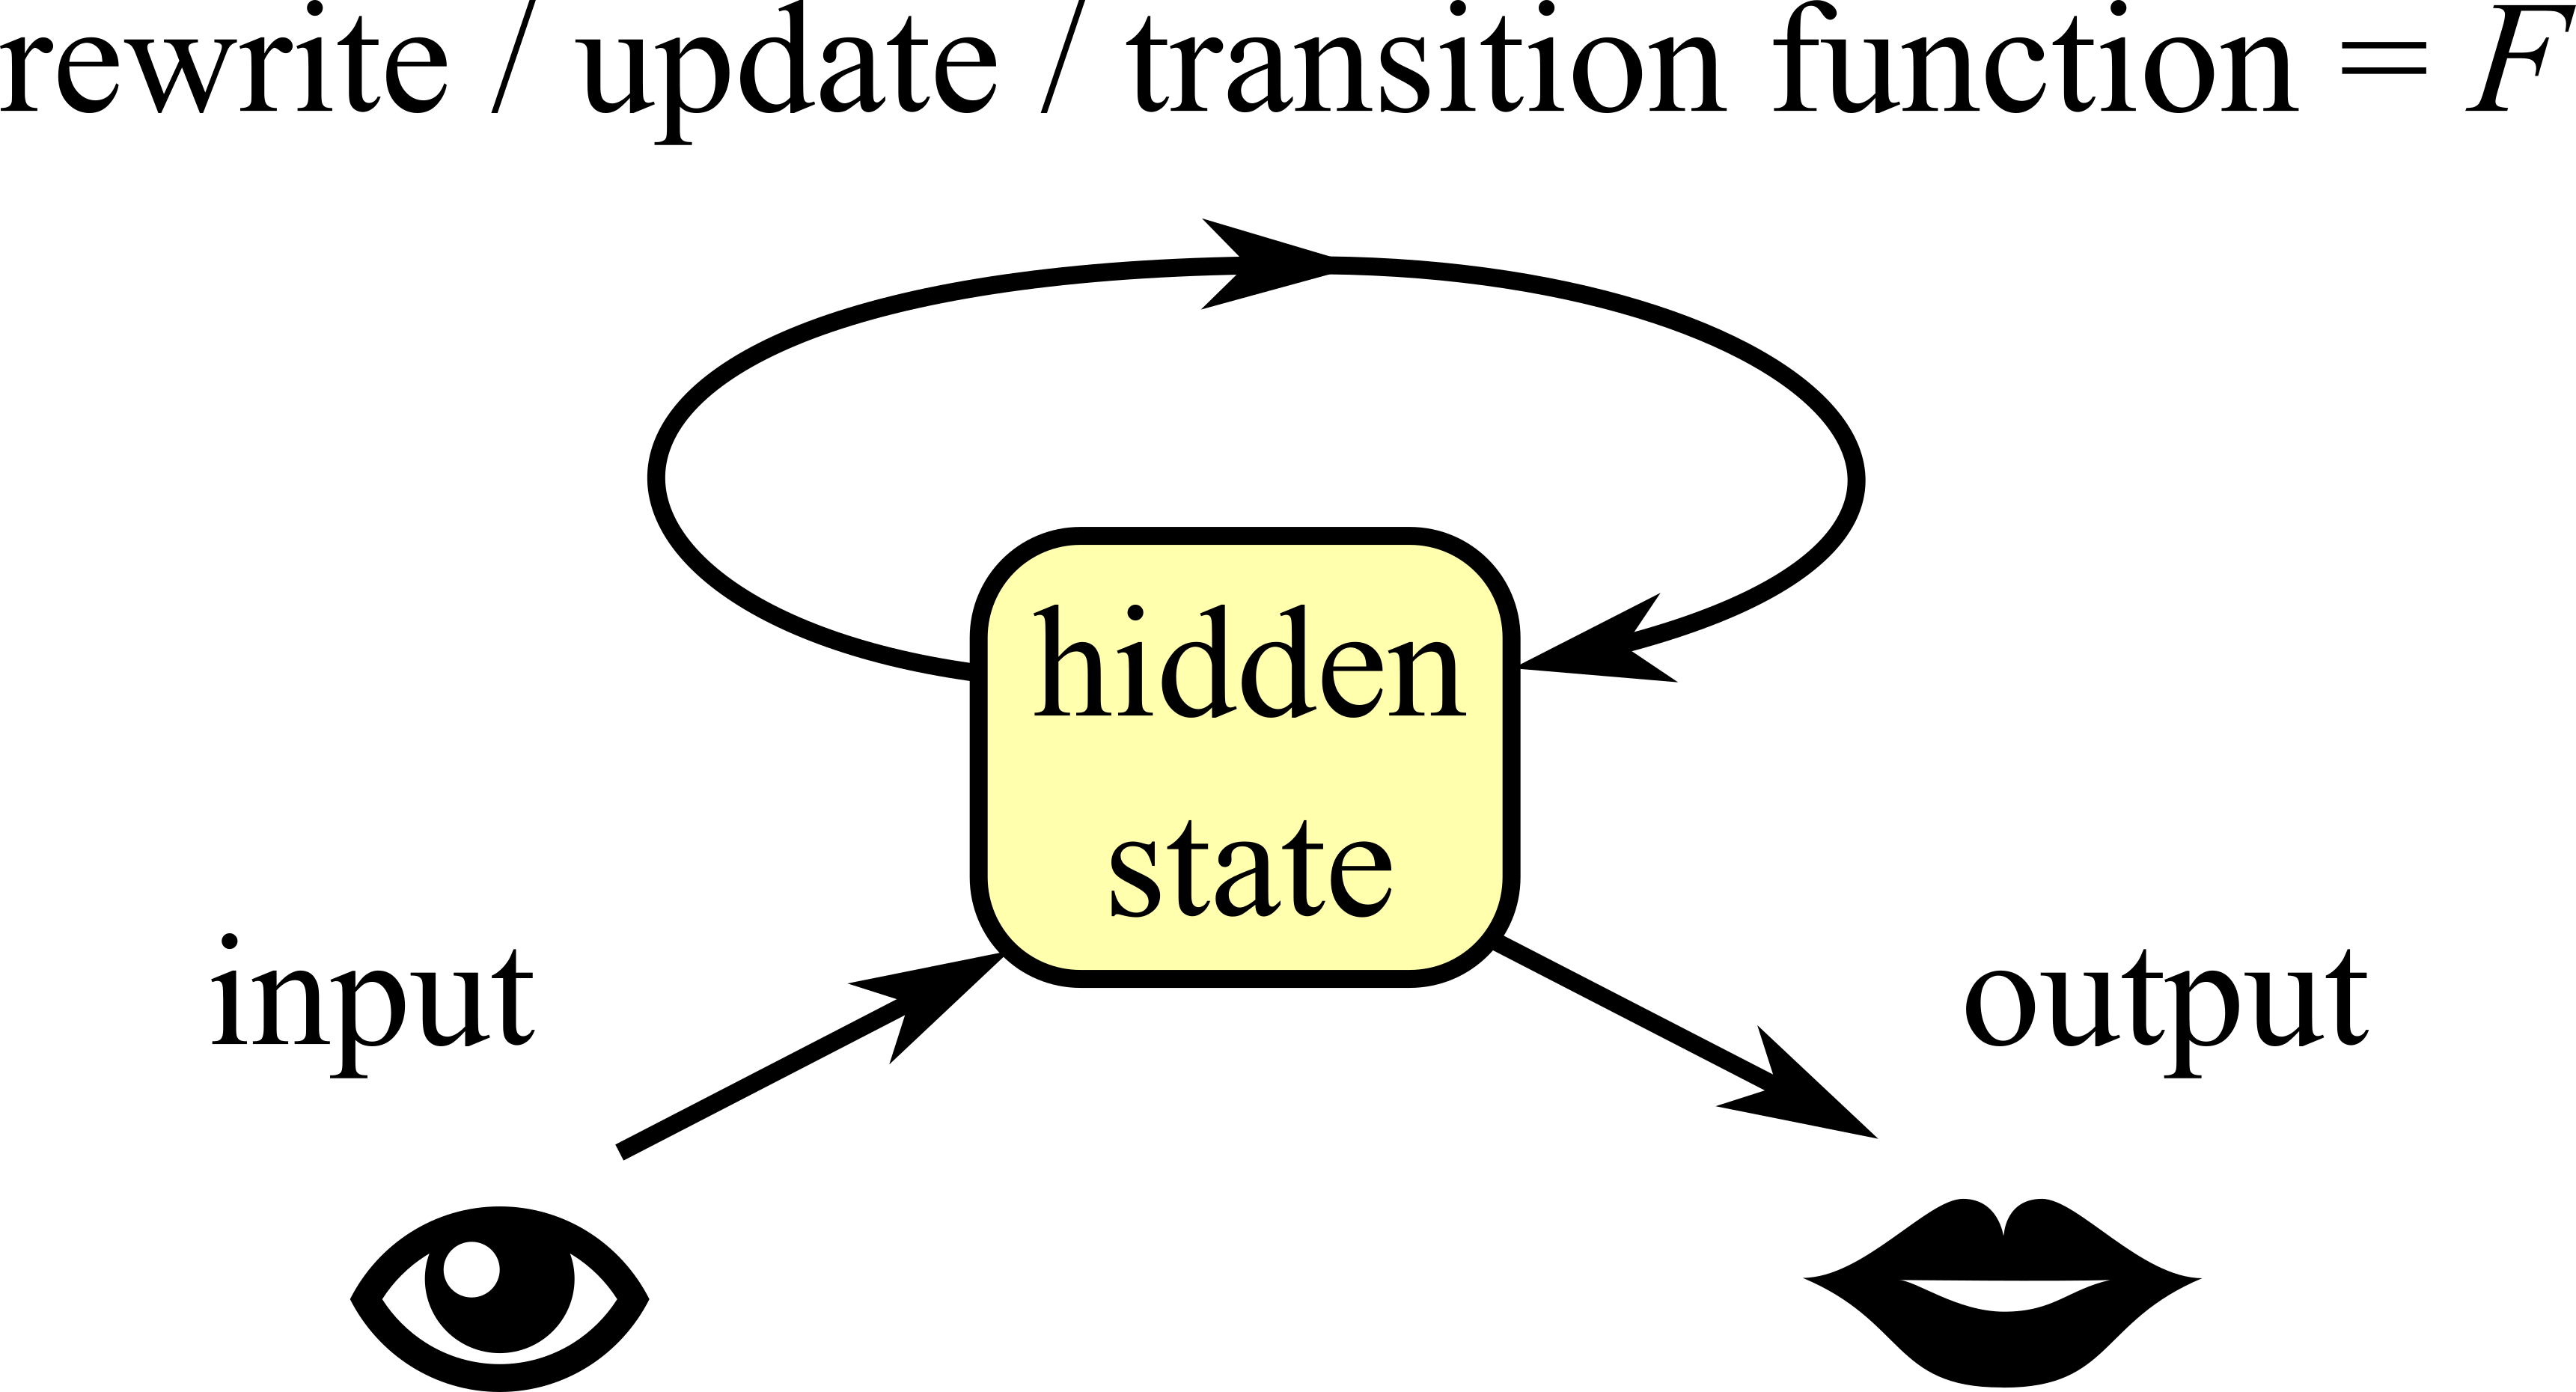
\includegraphics[scale=0.5]{minimal-architecture.png}}}
	\end{equation}

	\item \cc{
	它在 \textbf{强化学习} 的框架下,根据 Bellman 最优化条件,将 奖励 最大化}{
	It operates under reinforcement learning, maximizing rewards by the Bellman optimality condition
	}

	\item \cc{
	Transition function $F$ 可以用一个 神经网络 实现}{
	The transition function $F$ can be implemented by a neural network
	}
	
	\item \cc{
	根据我先前解释过的 no free lunch 理论,这个架构的问题是缺乏 inductive bias,学习太慢}{
	According to No Free Lunch theorem, problem with this architecture is lack of inductive bias, learning is too slow
	}
	
\end{itemize}
\end{frame}

\begin{frame}
\frametitle{\cc{No free lunch (NFL) 的迷思}{Some musings on No Free Lunch (NFL)}}
\begin{itemize}
	\item \cc{
	根据 no free lunch 哲学,没有所谓「好」与「坏」的归纳偏好}{
	According to NFL, there is no such things as ``good'' or ``bad'' inductive bias
	}

	\item \cc{
	只要能加速学习的,但又不完全 切掉 AGI,都是好 bias}{
	As long as it accelerates learning, and still accomodates AGI, it is good bias:
	}
	\begin{equation}
		\vcenter{\hbox{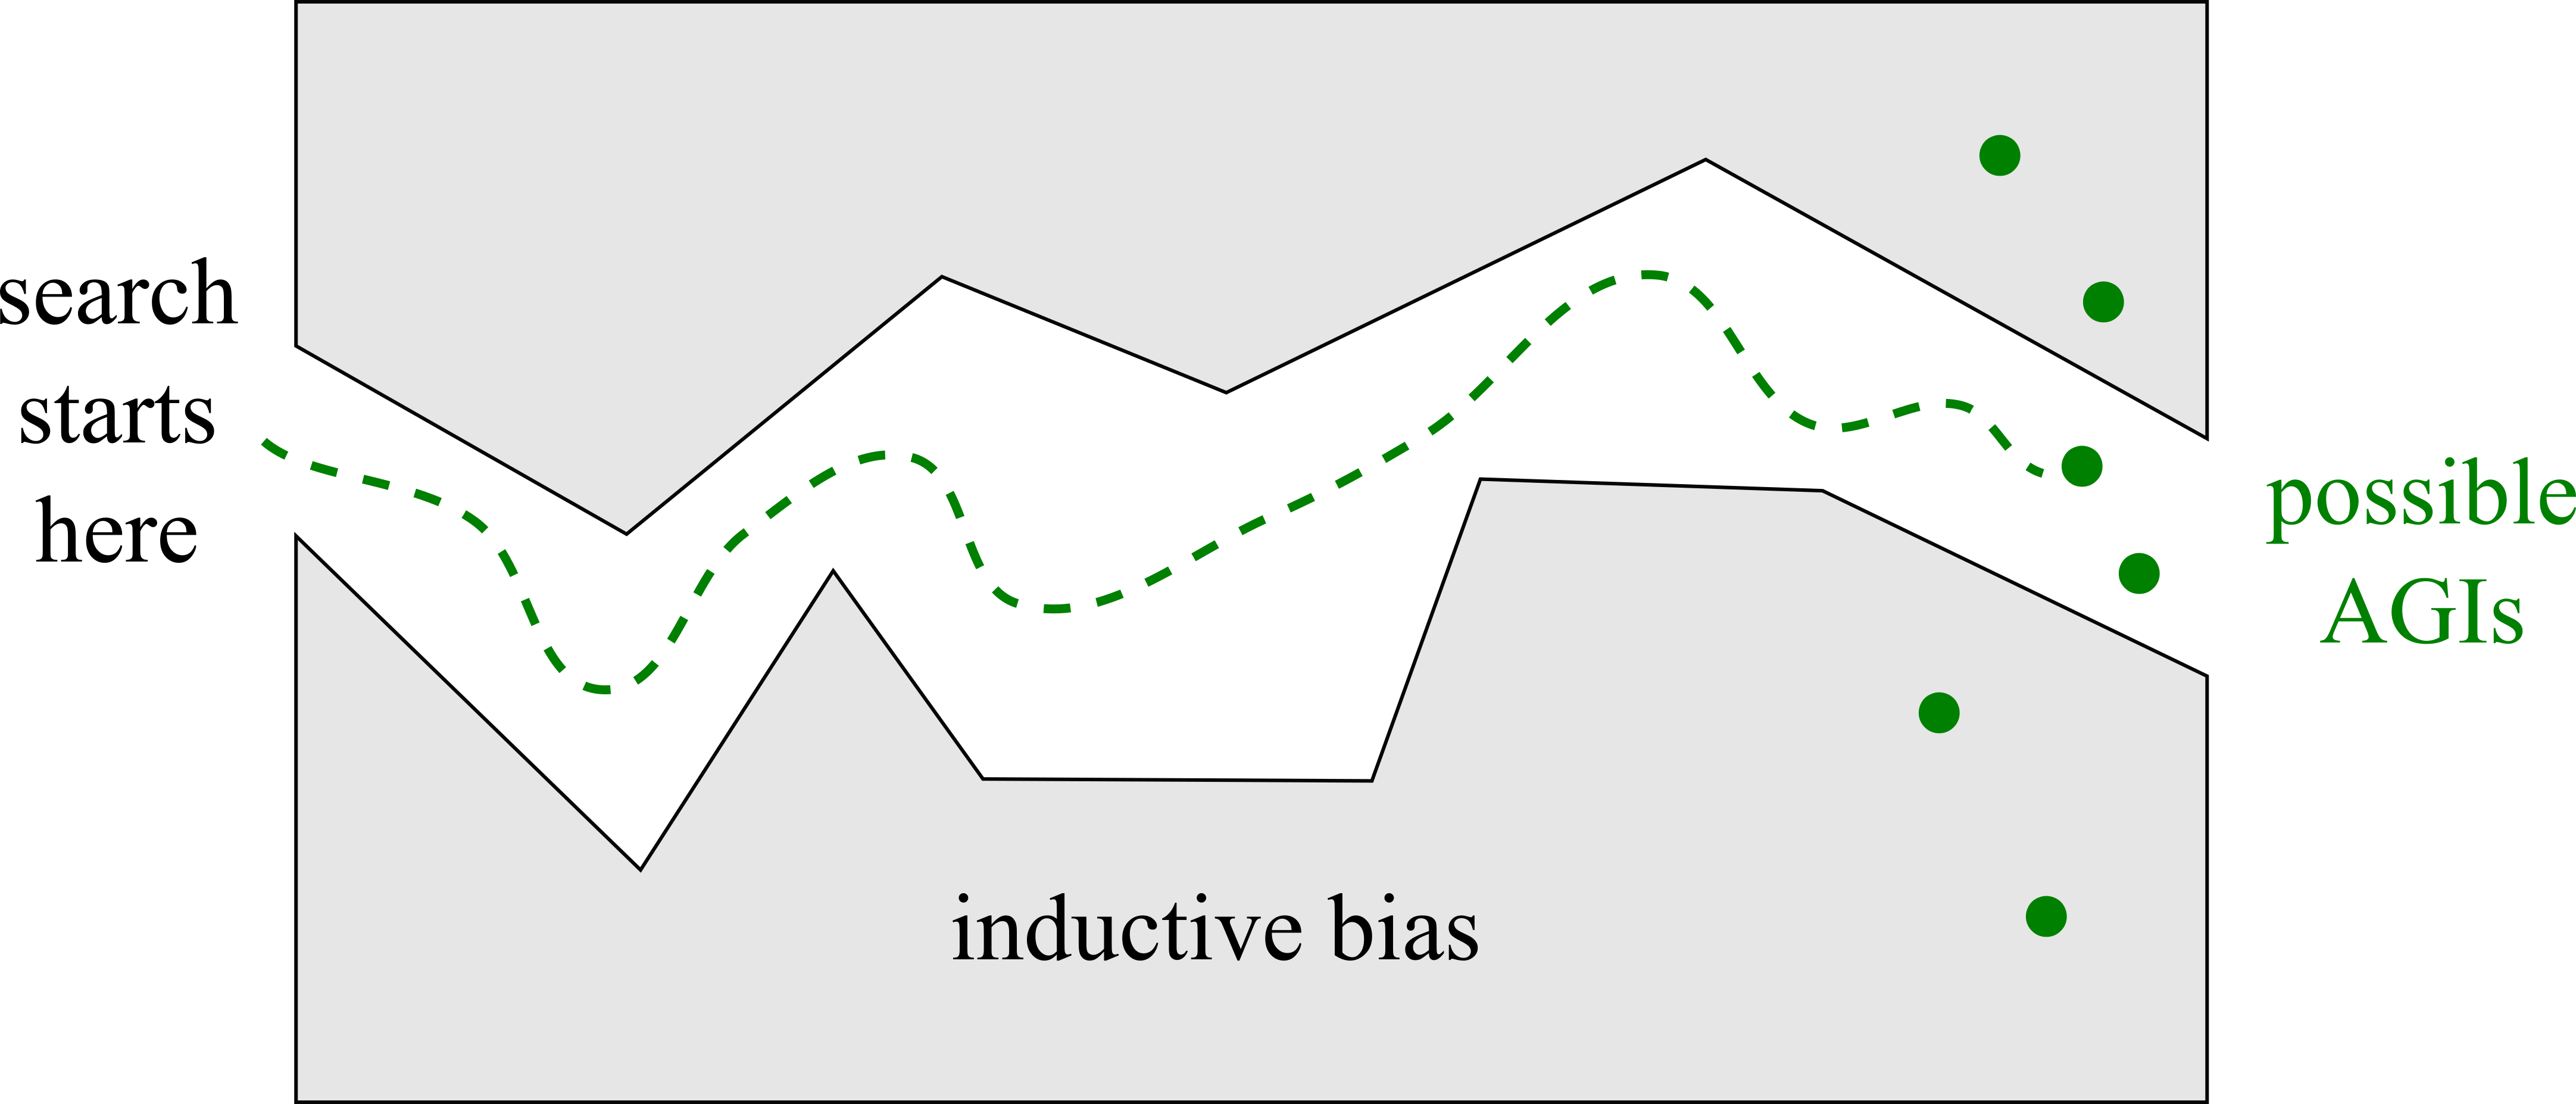
\includegraphics[scale=0.5]{no-free-lunch.png}}}
	\end{equation}

	\item \cc{
	例如,可以将 $F$ 的神经网络 变 \textbf{稀疏} (sparse),但保持 深度 (deep)}{
	For example, the neural network $F$ can be made \emp{sparse} while preserving deepness
	}
	
	\item \cc{
	但我之前提议用 \textbf{逻辑结构} 作为 bias,是否\red{多此一举}呢?! \confoundFace }{
	Yet, I proposed earlier to use logic as bias.  Is that redundant? \confoundFace
	}
\end{itemize}
\end{frame}

\begin{frame}
\frametitle{\cc{「双回路」架构}{``Double loop'' architecture}}
\begin{itemize}
	\item \cc{
	假设 working memory 是由分离的 \textbf{命题} (\red{\textbullet}) 构成的,可以提出一个「双回路」的架构: (这意思是,例如回路中载有10个命题,则它运转10次,隐状态即「浓缩」了这10个命题的资讯,然后输出一个新命题)}{
	Assume \emp{working memory} consists of disparate propositions (\red{\textbullet}), residing in an inner loop.  As this loop is iterated, the propositions are condensed into the hidden state.  Hence the ``double-loop'' architecture
	}
	\begin{equation}
	\vcenter{\hbox{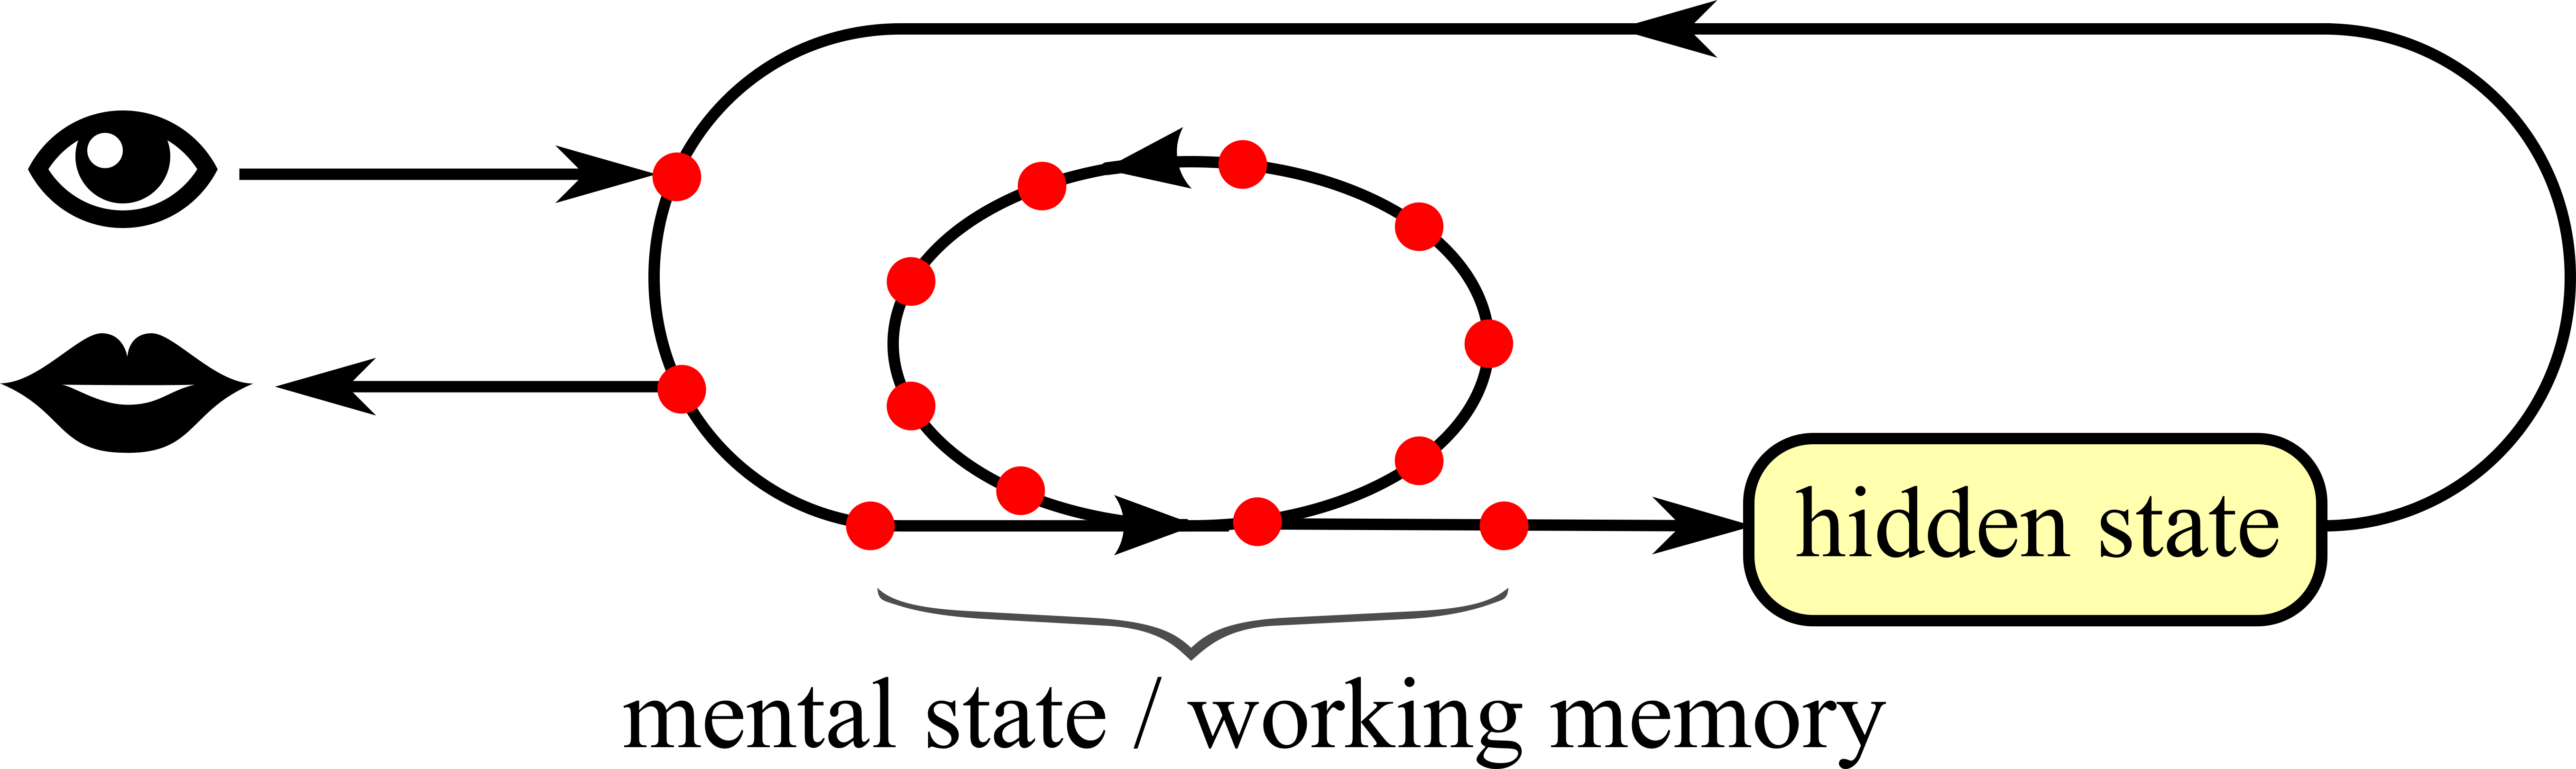
\includegraphics[scale=0.5]{double-loop-architecture.png}}}
	\label{double-loop-arch-1}
	\end{equation}

	\item \cc{
	这种架构很可能是人脑的架构,因为比较简单,可以进化出来}{
	This same architecture may be shared by the human brain, as its structure is simple and thus could have been evolved
	}

	\item \cc{
	据我所知,BERT 架构含有一个回路/一个隐状态 (BERT 逐个输入句子的单词,然后 隐状态 再将输出的单词 逐个吐出来)}{
	As far as I know, BERT also contains an implicit recurrence, where words in a sentence are condensed into a hidden state, from which target words are generated one by one
	}
	
	\item \cc{
	似乎 将 BERT 变成「双回路」,可以得到 AGI: (但我不熟悉 BERT)}{
	So it seems that if we modify BERT to be a ``double loop'', we can get an AGI:
	}
	\begin{equation}
		\boxed{\text{\cc{单词/概念}{words / concepts}}} \stackrel{\text{loop 1}}{\longrightarrow} \boxed{\text{\cc{句子/命题}{sentences / propositions}}} \stackrel{\text{loop 2}}{\longrightarrow} \boxed{\text{mental state}}
	\end{equation}
\end{itemize}
\end{frame}

\begin{frame}[plain]
% \frametitle{「双回路」架构}
\begin{itemize}
	\item \cc{
	图 (\ref{double-loop-arch-1}) 不够严谨,详细画出来是这样的:}{
	Diagram (\ref{double-loop-arch-1}) is a bit inaccurate, here is a more detailed diagram:
	}
	\begin{equation}
		\label{double-loop-arch}
		\vcenter{\hbox{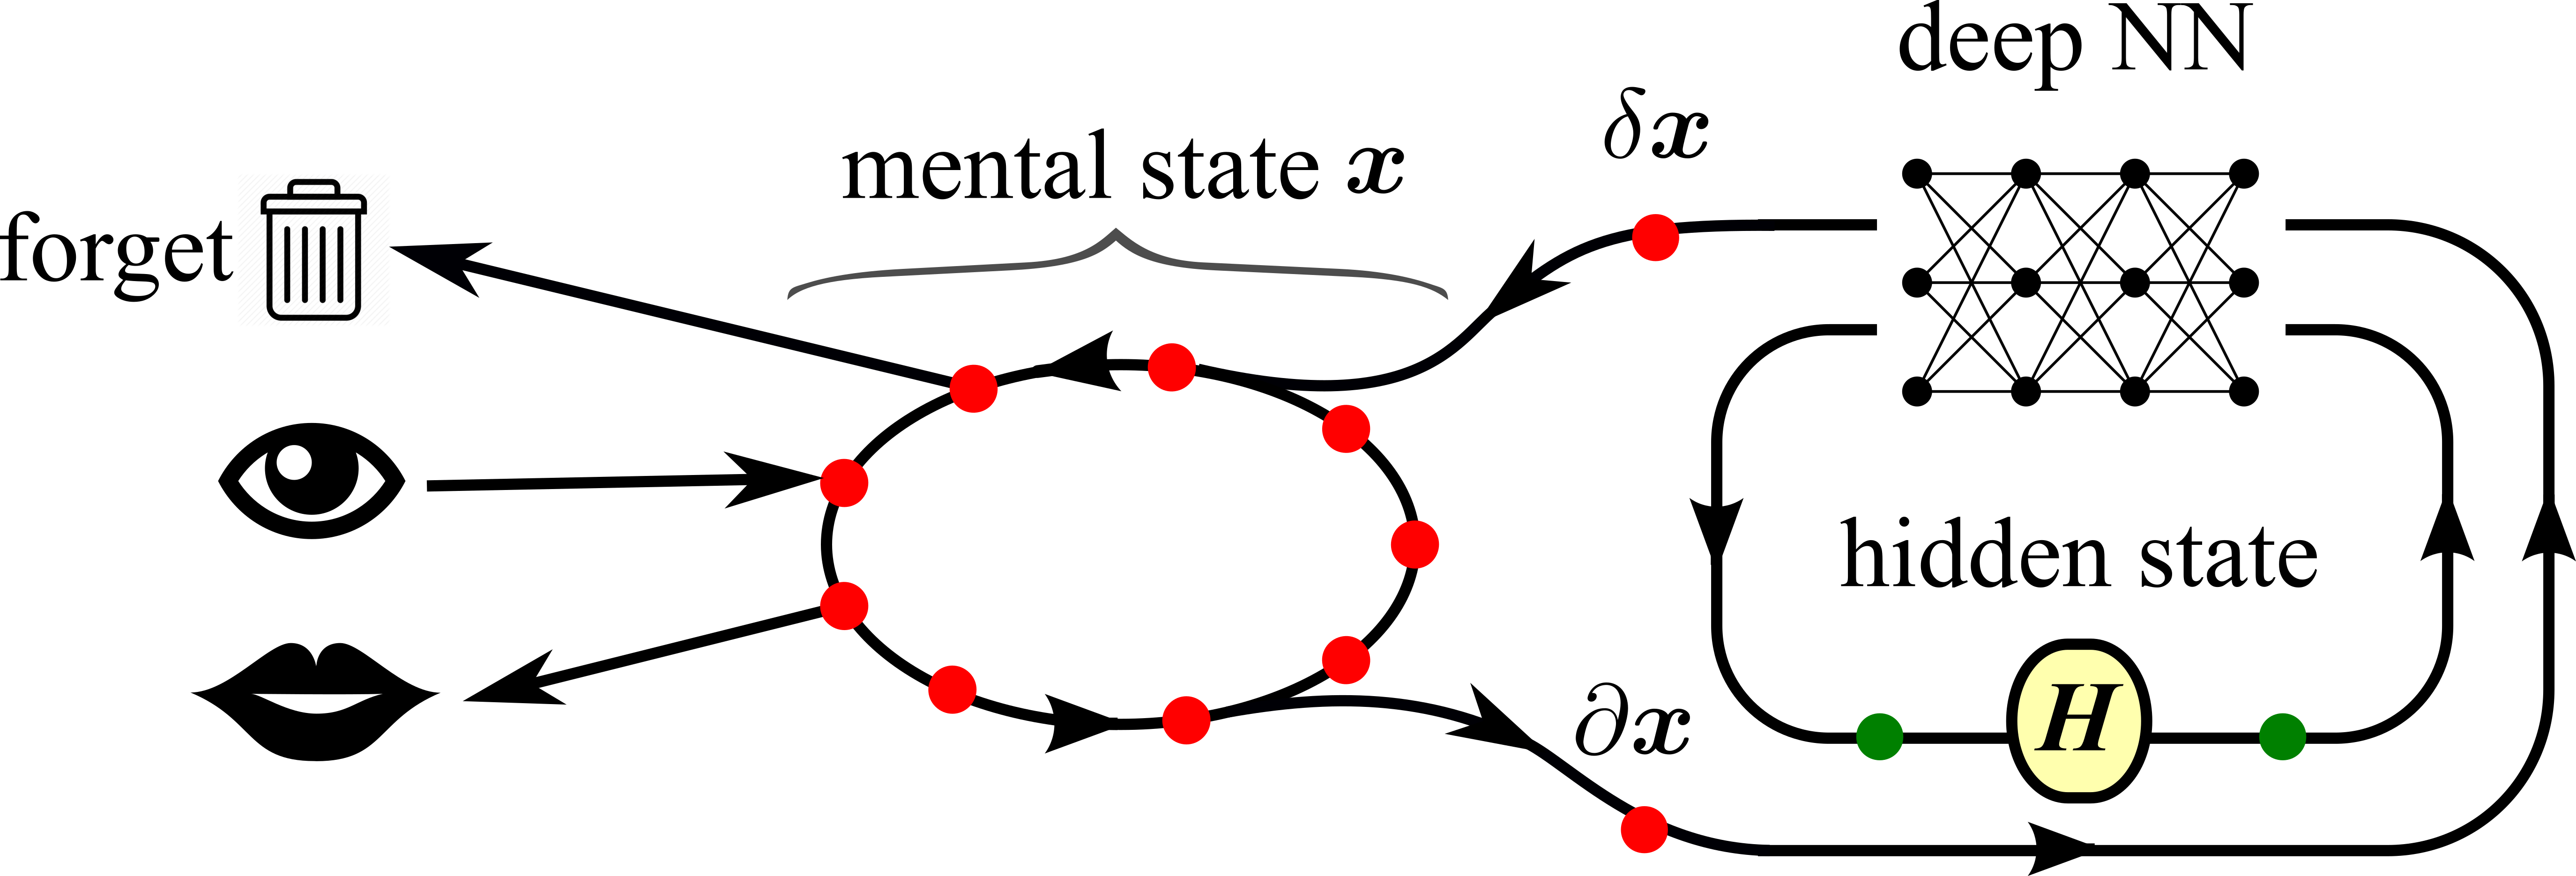
\includegraphics[scale=0.5]{double-loop-architecture-2.png}}}
	\end{equation}

	\item \cc{
	相比之下,如果用了 symmetric NN 则架构更简单:}{
	In contrast, one can use a \emp{symmetric NN} to make the architecture even simpler:
	}
	
	\begin{equation}
		\label{symNN-arch}
		\vcenter{\hbox{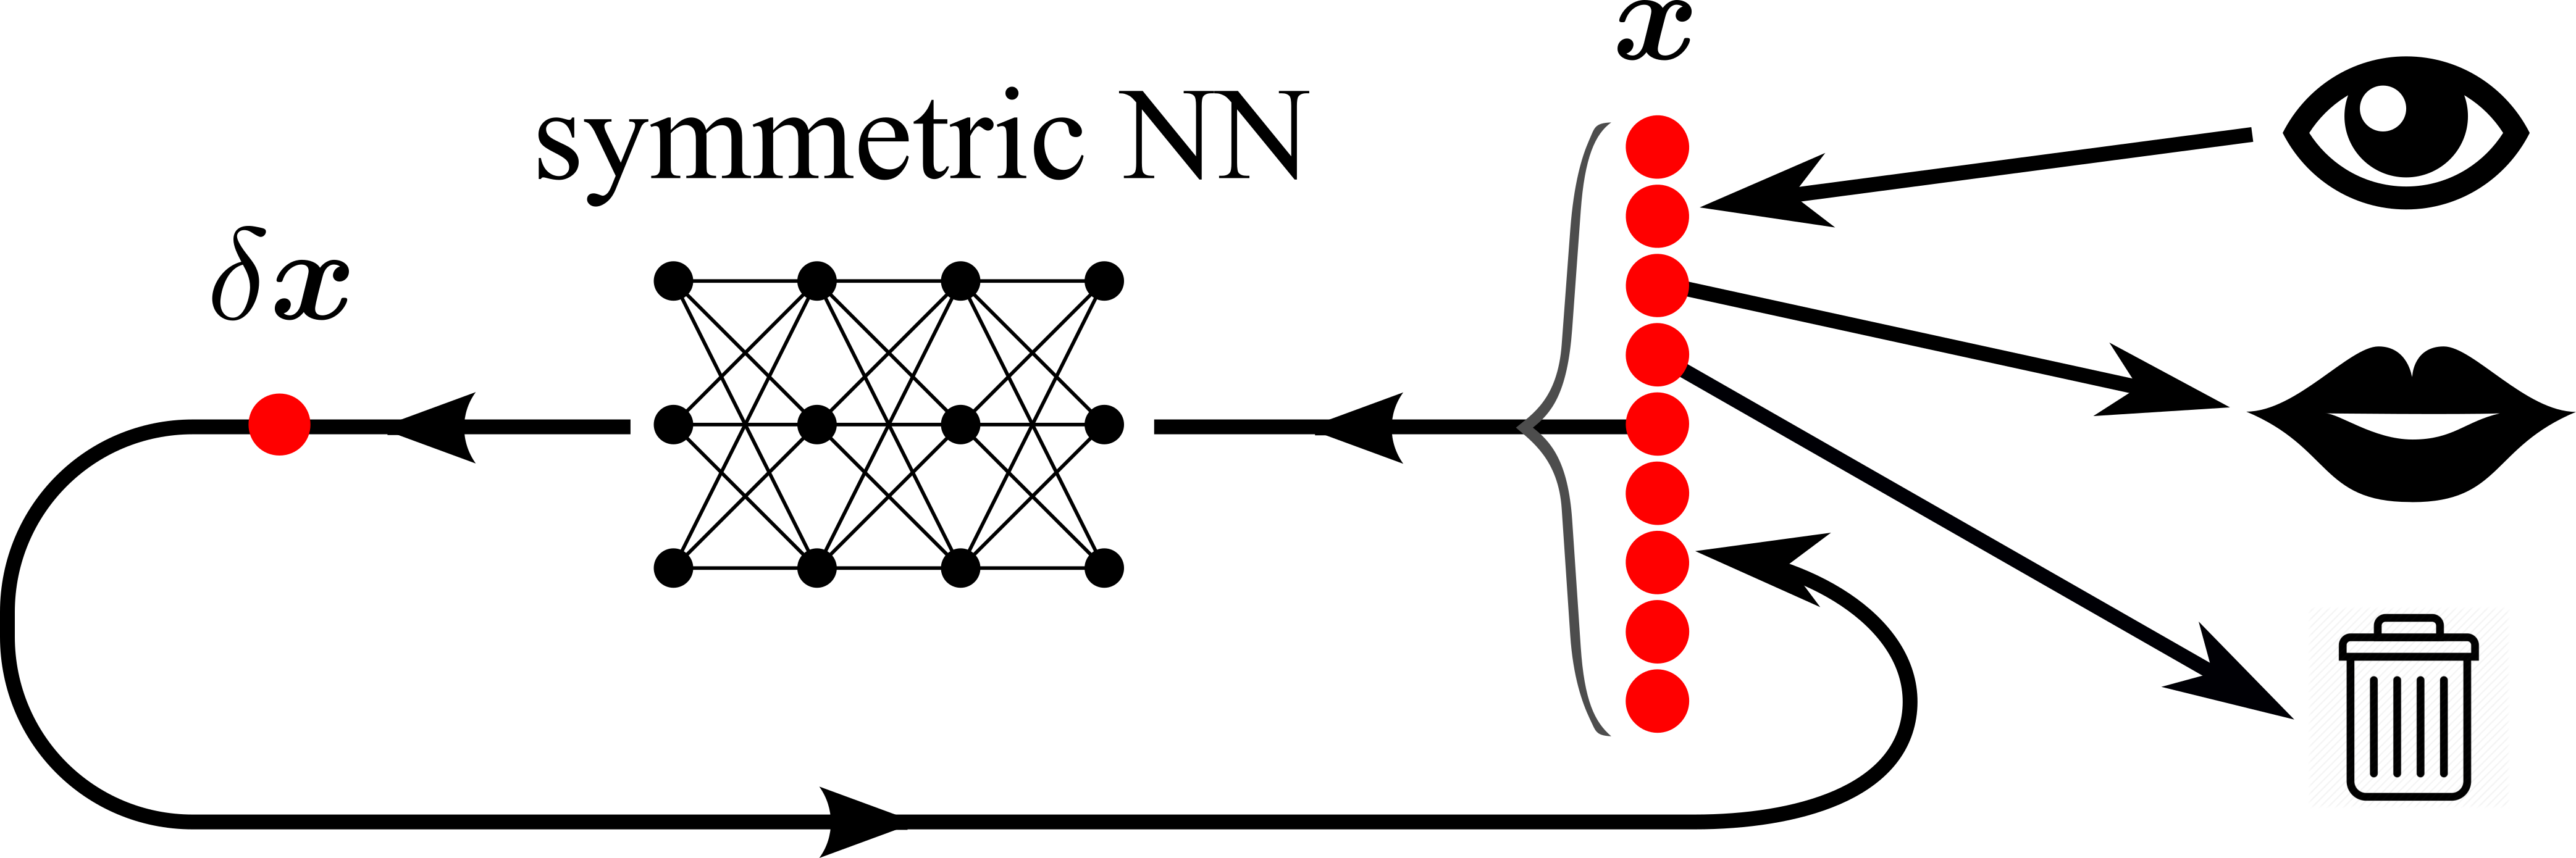
\includegraphics[scale=0.5]{symNN-architecture.png}}}
	\end{equation}

	\item \cc{
	问题是 (\ref{double-loop-arch}) 和 (\ref{symNN-arch}) 哪个的 学习速度 更快?  但不易判断 \confoundFace}{
	But it's not easy to decide whether (\ref{double-loop-arch}) or (\ref{symNN-arch}) learns faster \confoundFace
	}
	
\end{itemize}
\end{frame}

\begin{frame}
\frametitle{\cc{强化学习 与 量子力学 之间的联系}{Connection between reinforcement learning \& quantum mechanics}}

\begin{itemize}
	\item \cc{
	强化学习 的最优化条件是 \textbf{Bellman} 方程:}{
	The optimal condition for reinforcement learning is the \emp{Bellman} equation:
	}
		\begin{equation}
			\boxed{\mbox{Bellman}} \quad S_t(x) = \max_u \{ L(x,u) + \gamma S_{t+1}(x) \}
		\end{equation}
		
	\item \cc{
	而 Bellman 方程 的 微分形式,是经典分析力学中的 \textbf{Hamilton-Jacobi} 方程 (这点在 1970s 已经为 Kalman 和 Pontryagin 等人认识),现代叫这方程为 Hamilton-Jacobi-Bellman (HJB) 方程:}{
	The differential version of Bellman equation is the \emp{Hamilton-Jacobi} equation in classical analytic mechanics (This has been recognized in 1970's by Kalman, Pontryagin and others):
	}
		\begin{equation}
			\boxed{\mbox{Hamilton-Jacobi}} \quad \frac{\partial S(x, t)}{\partial t} = -H
		\end{equation}
		
	\item \cc{
	其中 Lagrangian $L$ 和 Hamiltonian $H$ 之间有关系:}{
	The Hamiltionian $H$ arises when trying to maximize the Lagrangian $L$ using Lagrangian multipliers.  Such multipliers have the interpretation of \emp{momentum}.
	}
	\begin{equation}
		L = \text{KE} - \text{PE} \quad , \quad H = \text{KE} + \text{PE}
	\end{equation}
	where $\text{KE}$ = kenetic energy, $\text{PE}$ = potential energy.

	\item \cc{
	至此,我们将一条 \textbf{离散}方程 变为 连续函数的\textbf{微分}方程,但\red{没有得益}}{
	Up to now, we changed a \emp{discrete} equation to a continuous \emp{differential} equation, but that has not yielded any advantage
	}
	
\end{itemize}
\end{frame}

\begin{frame}[plain]
\begin{itemize}
	\item \cc{
	我最近独立发现了从经典力学的 Hamilton-Jacobi 方程 过渡到 Schr\"{o}dinger 方程的 exact 形式,关键是透过 $\Psi = e^{-i \hbar S}$ 此一代入:}{
	Recently I independently discovered an exact way to go from the classical Hamilton-Jacobi equation to the Schr\"{o}dinger equation via the substitution $\Psi = e^{-i \hbar S}$:
	}
		\begin{equation}
		\boxed{\mbox{Hamilton-Jacobi}} \quad \frac{\partial S}{\partial t} = - H \quad
		\Rightarrow
		\quad i \hbar \frac{\partial \Psi}{\partial t} = H \Psi \quad \boxed{\mbox{Schr\"{o}dinger}}
		\end{equation} 
		
	\item \cc{
	一直以来,量子力学的教科书 认为这种 量子化 (quantization) 过程 只能够是近似性的。  后有朋友告诉我 \parencite{Field2010} 已导出了这结果。}{
	We have always been told in textbooks that such a process of \emp{quantization} can only be achieved heuristically, but some friend informed me that \parencite{Field2010} has derived this result.
	}
	
	\item \cc{
	从 AI 的角度来看,这结果表示: \red{强化学习 可以 转化为 在 Hilbert 空间中求解 Schr\"{o}dinger 方程!}}{
	From the perpective of AI, this means that \red{solving the reinforcement learning problem is equivalent to solving the Schr\"{o}dinger equation in Hilbert space!}
	}
	
	\item \cc{
	而,Schr\"{o}dinger 方程可以透过 \textbf{虚数时间} (imaginary time) 转化为 热力学的 \textbf{扩散} (diffusion) 方程}{
	Moreover, the Schr\"{o}dinger equation can be transformed into the \emp{diffusion} / heat equation via the introduction of \emp{imaginary time}:
	}
		\begin{equation}
			\boxed{\mbox{wave eqn.}} \quad \frac{\partial \Psi}{\partial t} + i \Delta \Psi = 0
			\quad \leftrightsquigarrow \quad
			\frac{\partial u}{\partial t} + \Delta u = 0 \quad \boxed{\mbox{heat eqn.}}
		\end{equation}

	\item \cc{
	但应用到 AI 上需要 \textbf{离散化},特别是利用 discrete Laplacian $\Delta$ 或 discrete Schr\"{o}dinger operators 作用在 \red{graph} 上(状态空间是 graph)}{
	Yet, if this is to be applicable to AGI, we need to \emp{discretize} the state space (which becomes a graph), and use the discrete Laplacian $\Delta$ or discrete Schr\"{o}dinger operator to act on graphs
	}
	
	\item \cc{
	暂未知这方向有没有好处 \confoundFace}{
	Impressive as it may sound, this may be of low practical value \confoundFace
	}
	
\end{itemize}
\end{frame}

\begin{frame}
\frametitle{\cc{Topos 理论}{Topos theory}}

\cc{
Topos 是指一个能够在里面「\red{做逻辑}」的范畴,它起源於 Lawvere 于 1950s 将 \textbf{集合论} 表述成 \textbf{范畴论} 的尝试。 \\}{
A topos is a category in which one can ``\red{do logic}''.  The idea originated in 1950's when Lawvere tried to re-formulate the foundation of mathematics / \emp{set theory} in the new language of \emp{category theory}. \\
}
\cc{
在一个 topos 范畴内的物体 (objects) 可以进行三种运算:}{
In a topos, 3 operations are allowed between objects:
}
\begin{itemize}
	\item Cartesian product $A \times B$ \cc{
	(对应命题逻辑的 $A \wedge B$)}{
	(corresponding to $A \wedge B$ in propositional logic)
	}
	\item exponentiation $A \rightarrow B = B^A$ \cc{
	 (对应命题逻辑的 $A \Rightarrow B$)}{
	(corresponding to $A \Rightarrow B$ in propositional logic)
	}
	\item subobject classifier $A \hookrightarrow B$  \cc{
	(表示 \textbf{子集} $A \subseteq B$ 的概念)}{
	(corresponding to the subset notion $A \subseteq B$)
	}
\end{itemize}
\cc{
Topos 理论的重要性在於: 它概括了哪些数学结构有进行 \textbf{逻辑} 的能力,例如一些 relation graphs,algebras 等。 \\}{
The significance of topos theory is that it distills which mathematical structures are able to carry on \emp{logic} operations, e.g. relation graphs, algebras, etc. \\
}
\cc{
在我的理论里,神经网络 $F$ 负责 $U \stackrel{F}{\rightarrow} V$ 即 exponentiation $V^U$ 这部分,而 $U, V$ 是向量空间。 这至少要求我们将 $A \times B$ 的结构 embed 到向量空间中。 由於 $A \times B = B \times A$ 是\textbf{可交换}的,这促使我看了一下 Abel 群的理论。}{
In my theory, the neural network $F$ implements $U \stackrel{F}{\rightarrow} V$ which is the exponentiation $V^U$, where $U, V$ are vector spaces.  This requires, at least, to embed the structure of $A \times B$ into vector space.  However $A \times B = B \times A$ is \emp{commutative}, which led me to consider Abelian group theory....
}
\end{frame}

\begin{frame}
\frametitle{\cc{交换不变性 (permutation invariance)}{Permutation invariance}}
\begin{itemize}
	
	\item \cc{
	最近有個颇厉害的想法,将 Word2Vec 嵌入到 Poincar\'{e} disc / hyperbolic space \parencite{Nickel2017}}{
	Recently a nice idea has been proposed to embed Word2Vec into Poincar\'{e} disc / hyperbolic space \parencite{Nickel2017}
	}
	
	\item \cc{
	类似地,能不能将 逻辑物体 的 vectors 嵌入到 hyperbolic space? }{
	Can we similarly embed logic structures (as vectors) into hyperbolic space?
	}
	
	\item \cc{
	自由群 $F_2$ 的 Cayley 图是\textbf{树},但 \red{交换}自由群的 Cayley 图是\textbf{格状}的: }{
	Cayley graph of the free group $F_2$ is a \emp{tree}, but Cayley graph of the \red{Abelian} free group is \emp{grid}-like:
	}
		\begin{equation}
		\vcenter{\hbox{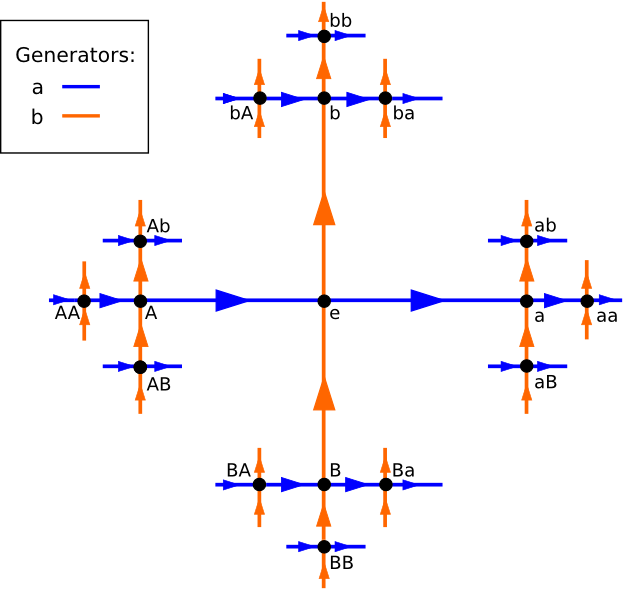
\includegraphics[scale=0.3]{Cayley-graph-F2.png}}}
		\quad \quad \quad
		\vcenter{\hbox{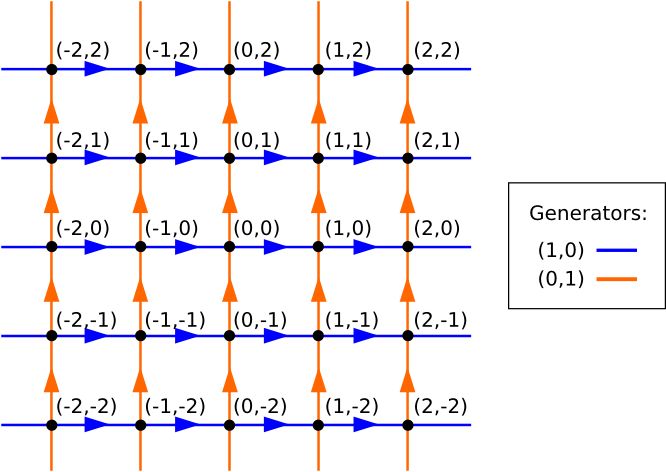
\includegraphics[scale=0.3]{Cayley-graph-Z2.png}}}
		\end{equation}
		
	\item \cc{
	一般来说,自由群 $F_n$ 的 Cayley 图可以嵌入到(平面的)hyperbolic disc 上,但 $F_n$ 的 Abelianization $F_n^{\text{Ab}} \cong \mathbb{Z}^n = \mathbb{Z} \times ... \mathbb{Z}$ 是一个 \red{$n$-维} 空间的 grid,似乎不可能嵌入到平面上}{
	Generally, the free group $F_n$'s Cayley graph can be embedded into the (planar) hyperbolic disc, but the Abelianization of $F_n = F_n^{\text{Ab}} \cong \mathbb{Z}^n = \mathbb{Z} \times ... \mathbb{Z}$ is a \red{$n$-dimensional} grid, which seems impossible to embed on a plane.
	}
	\item \cc{
	就算考虑 表示论 (representation theory),所有 Abel 群的不可约复表示 都是 1-维的。 $F_n^{\text{Ab}}$ 的表示,恰好是 $n$ 个 1-维 表示的直和。 没卵用!}{
	Even considering representation theory, all irreducible representations of Abelian groups are 1-dimensional.  The representation of $F_n^{\text{Ab}}$ is precisely the direct sum of $n$ copies of dim-1 representations.  Useless!
	}
	
\end{itemize}
\end{frame}

\begin{frame}[plain]
% \frametitle{交换不变的 神经网络}
\begin{itemize}
	% \item 就算考虑 表示论 (representation theory),所有 Abel 群的不可约复表示 都是 1-维的。 $F_n^{\text{Ab}}$ 的表示,恰好是 $n$ 个 1-维 表示的直和。 没卵用!
	\item \cc{
	上页结论是: $\mathbb{Z}^n$ 不可能嵌入到更低维的空间内,除非使用某种 \red{fractal} 方法。  然而,fractals 恰好是 神经网络 这件武器的「射程范围」之外! }{
	Seems that $\mathbb{Z}^n$ cannot be embedded into lower dimensions, unless we use some kind of \emp{fractal} structure.  However, fractals are exactly the realm that is out-of-reach of the universal approximating power of neural networks!
	}
	
	\item \cc{
	换个想法,通过 类似 weights-sharing 的 \textbf{约束},令 神经网络 变成 permutation invariant (= \red{Symmetric NN})}{
	Another strategy is to create \emp{symmetric} neural networks whose output is invariant when the input is permuted.  This could be achieved by ``weight-sharing''.
	}
	
	
	\item \cc{
	这方法 必需设 activation function = polynomial}{
	For this to work, the activation function must be \emp{polynomials}.
	}
	
	\item \cc{
	缺点是: 约束的数量 随著 层数 增加而 指数式增长,暂时只能做 1-2 层的,每层 = 2次多项式}{
	A drawback of this approach is when \# layers grow, \# constraints also grow exponentially, making it hard to build deep (many-layer) networks
	}

	\item \cc{
	优点是: 反正我们希望 神经网络 是 sparse(减少权重空间的自由度),而这个做法同时具有逻辑 bias}{
	An advantage is that the resulting NN is very sparse in terms of \# weights.  This is a form of inductive bias.
	}
	
	\item \cc{
	细节我会在另一篇论文讲述}{
	As of this writing, I am yet exploring another approach that is inspired by Google's BERT.  More on this later.
	}

\end{itemize}
\printbibliography
\begin{center}
	\cc{多谢收看}{Thanks for watching} \smiley
\end{center}
\end{frame}

\begin{comment}

\begin{frame}
\frametitle{References}
\footnotesize{
\begin{thebibliography}{99} % Beamer does not support BibTeX so references must be inserted manually as below
\bibitem[]{} Bart Jacobs (1999)
\newblock Categorical logic and type theory
% \newblock \emph{North Holland, Studies in logic} v141.

\bibitem[]{} Robert Goldblatt (2006)
\newblock Topoi -- the categorical analysis of logic

\end{thebibliography}
}
\end{frame}

\end{comment}

\end{document} 